\documentclass[12pt,a4paper]{article}
\usepackage[UTF8]{ctex}
\usepackage{amsmath}
\usepackage{graphicx}
\usepackage{makecell}
\usepackage{verbatim}
\usepackage[backref]{hyperref}
\author{刘润}

\begin{document}
\title{多DFT16模块并行的说明}
\maketitle

对于512点FFT,我们可以采用混合基分解的方式将其转变为两级DFT16,图1和图2展示了这种拆分方法。

\begin{figure}[htbp]
\centering
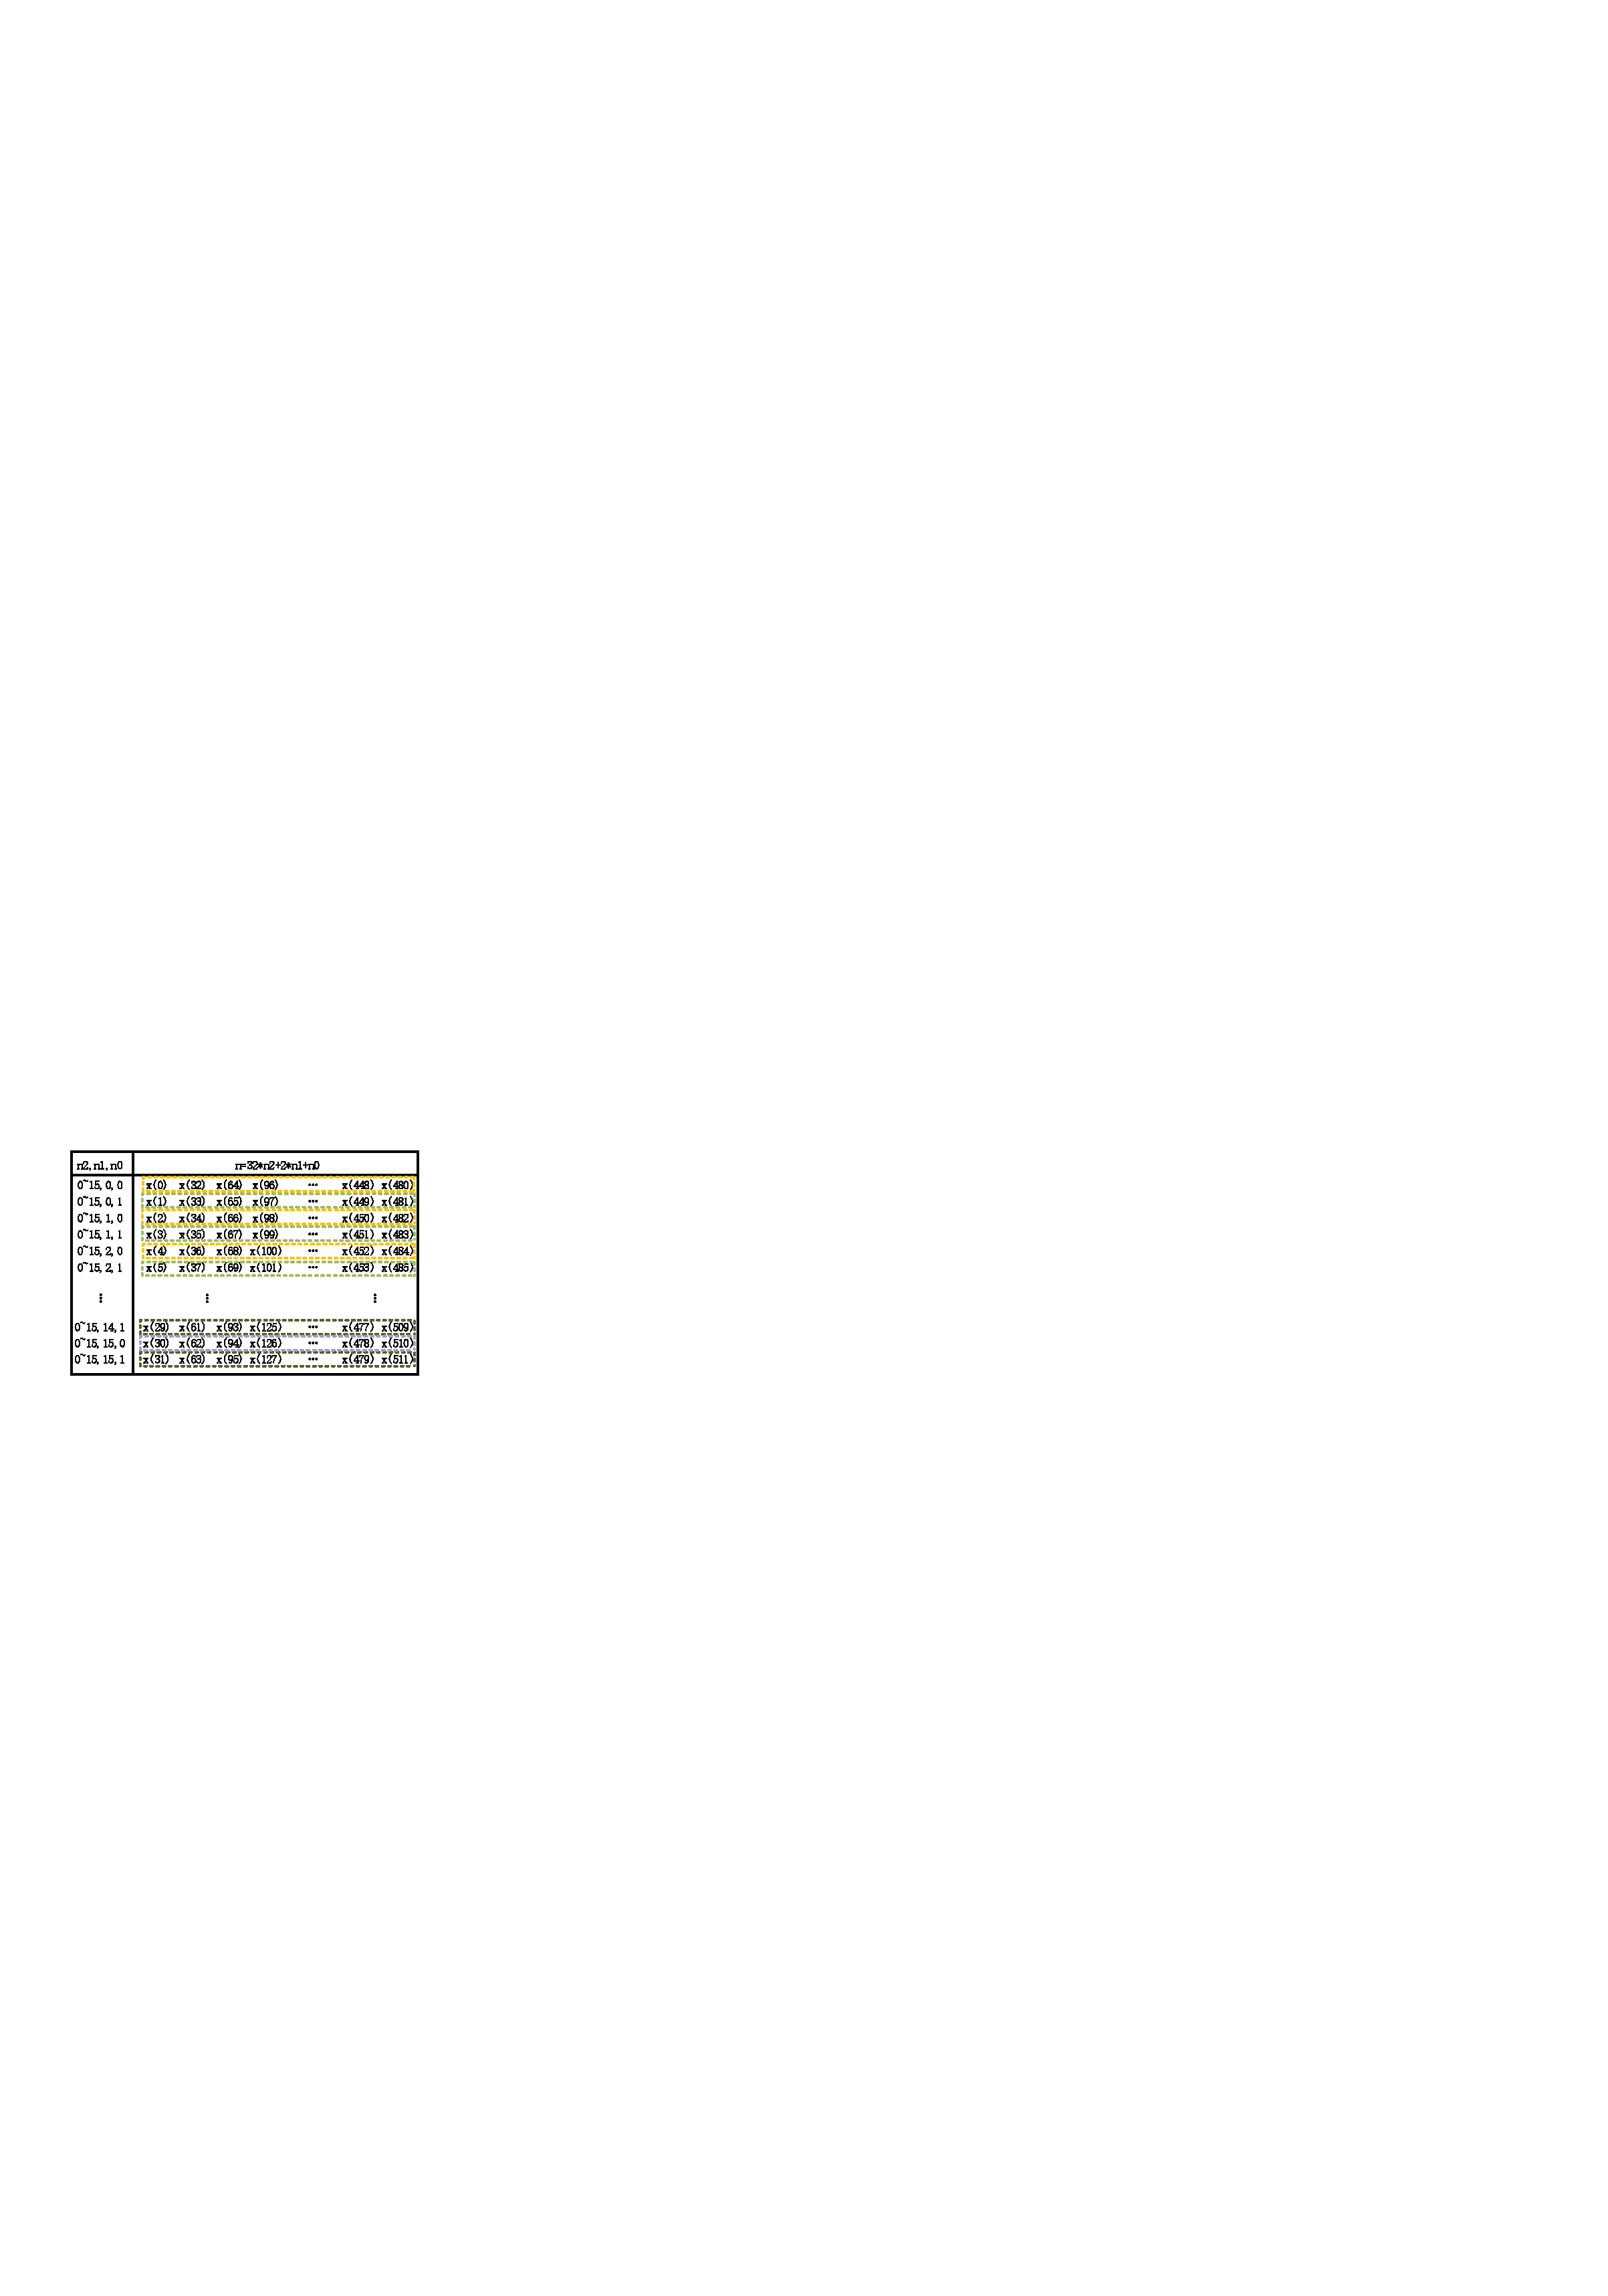
\includegraphics[scale=1.5]{figure/figure1}
\caption{第一级DFT16}
\end{figure}

\begin{figure}[htbp]
\centering
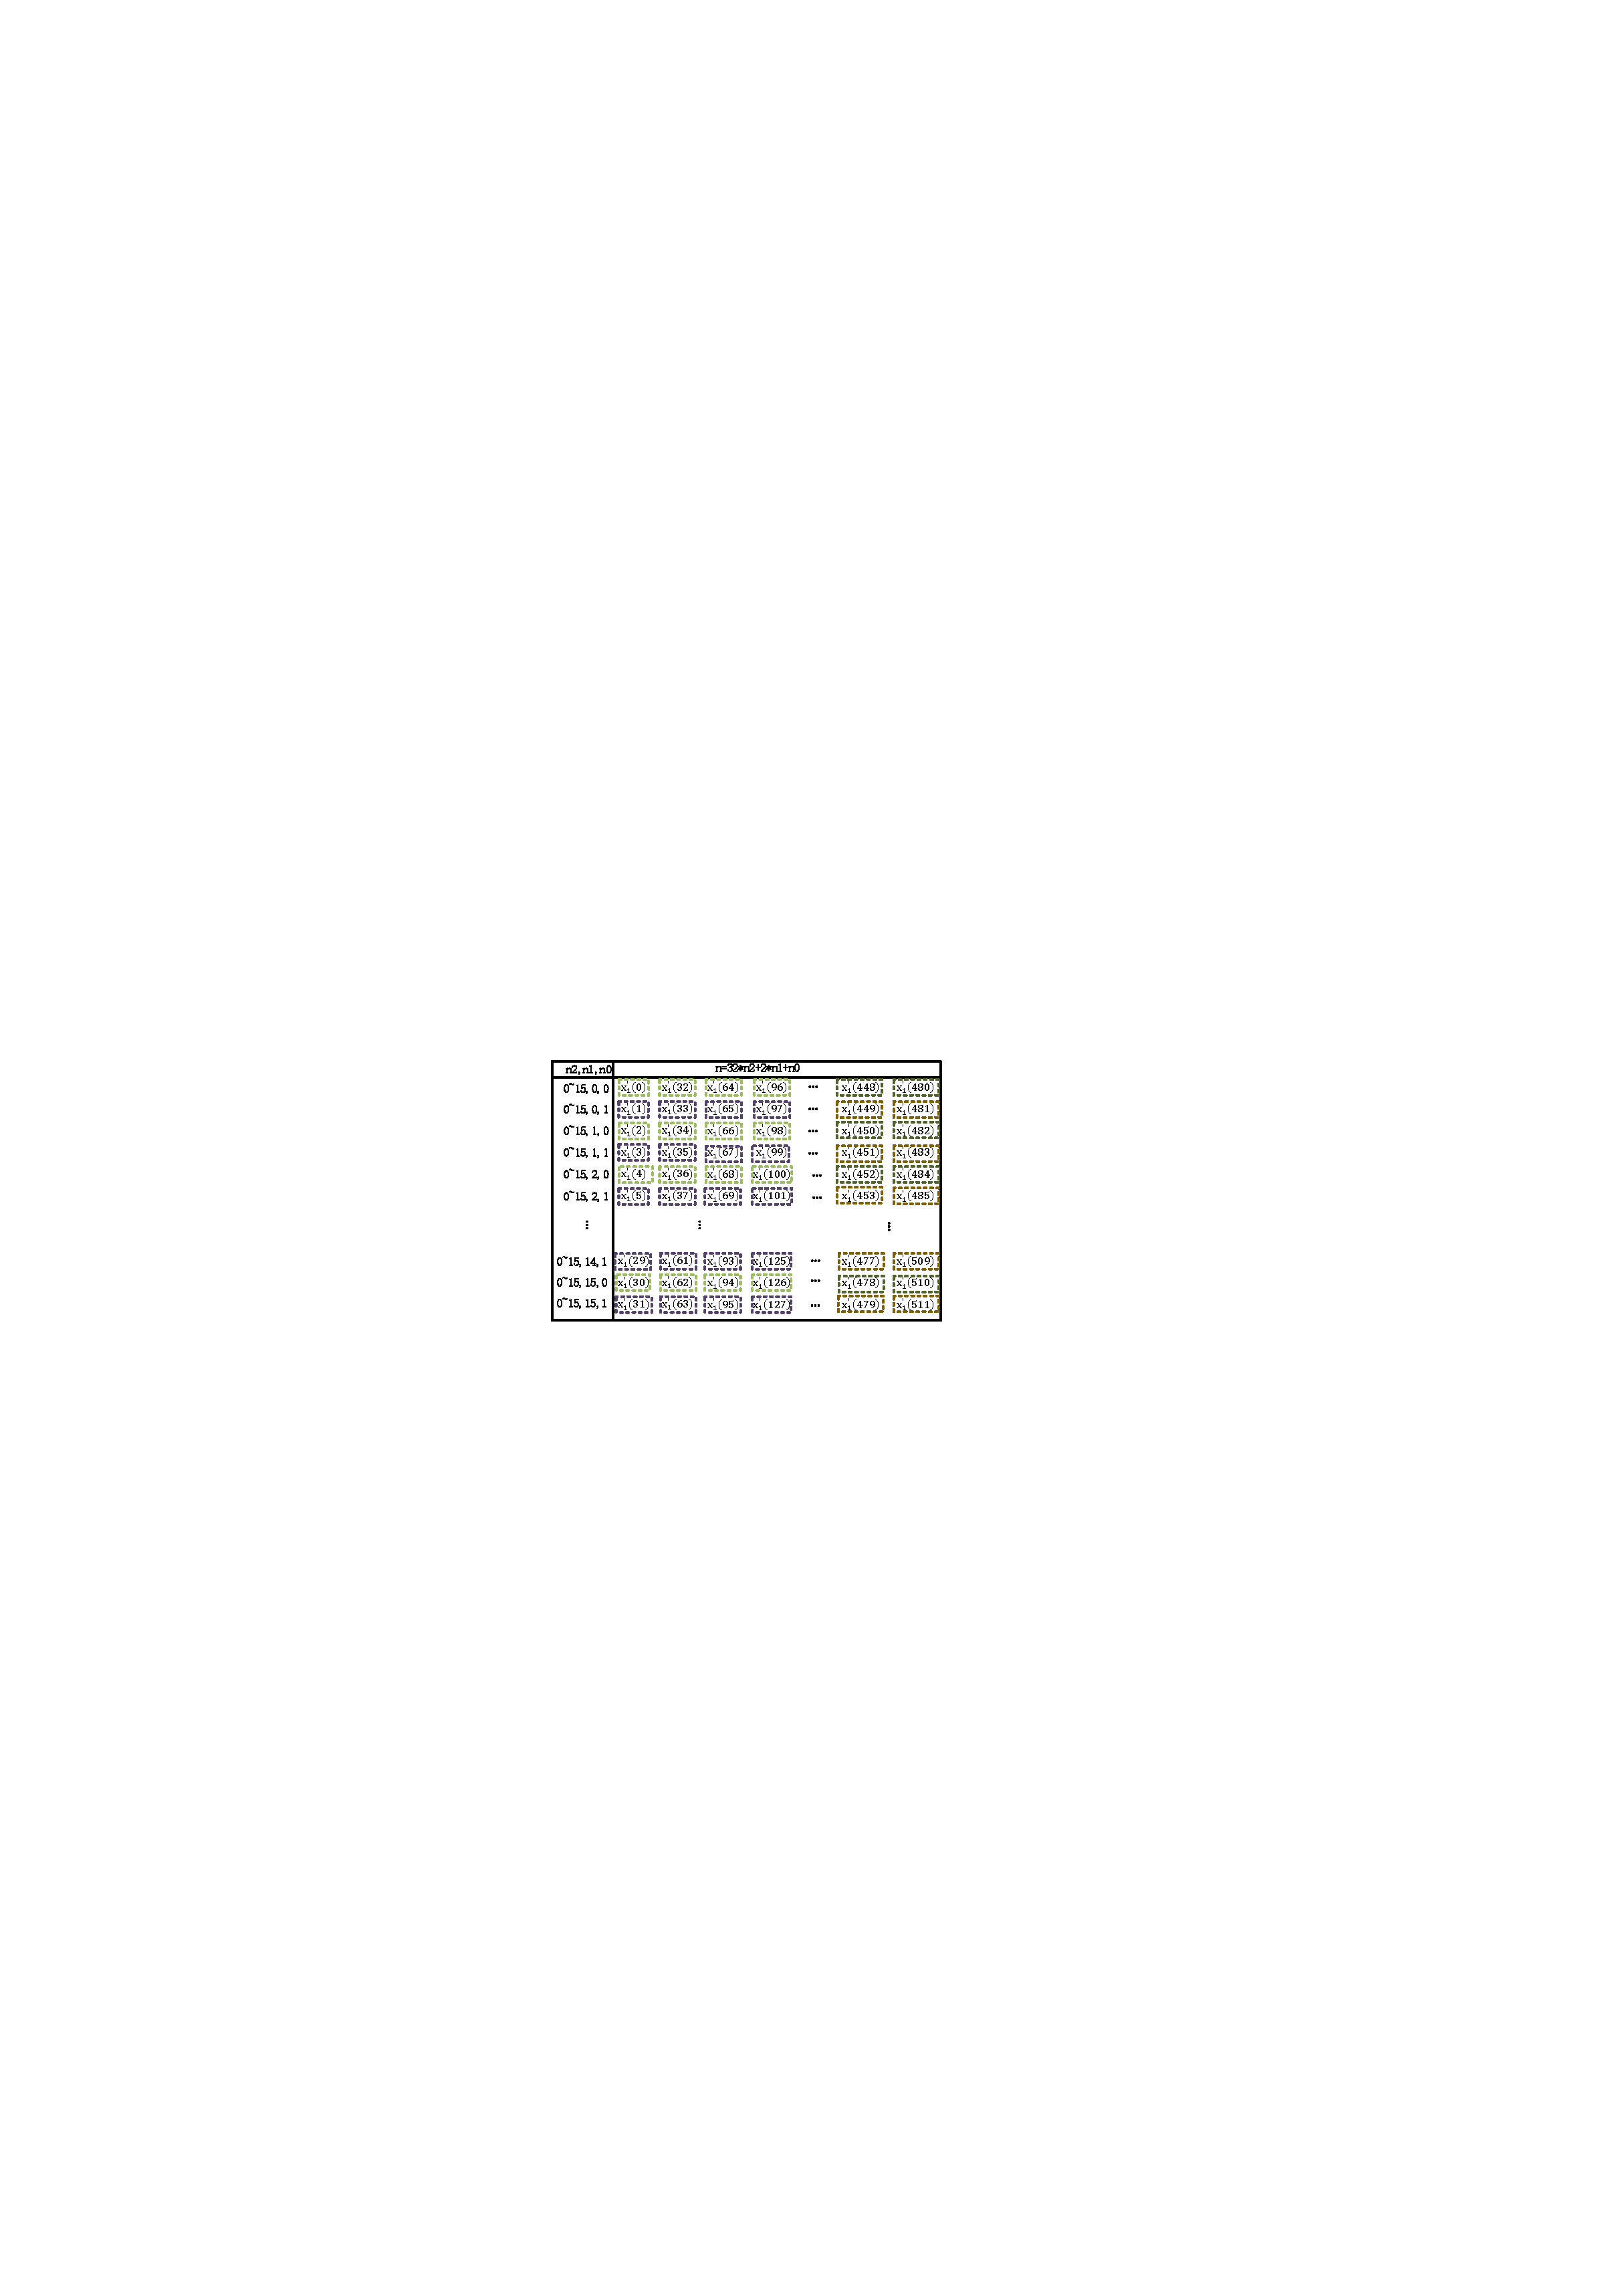
\includegraphics[scale=1.5]{figure/figure2}
\caption{第二级DFT16}
\end{figure}

从图1和图2中可以看出混合基分解之后的DFT16计算具有并行性,所以在存内计算的阵列中多个DFT16模块可以
并行计算,用以加快计算速度。在图3中,每一个方块代表一个DFT16模块,而同一种颜色的DFT16模块将会同时
运行,得到16个并行输出的结果。在图4中,给出了512点FFT分解为两级DFT16之后计算的时序图。在图4中,
每一个小方格代表一个DFT16模块,只有带有颜色的小方格才会处于计算状态,其余DFT16模块处于关闭状态。
在前四个小图中,每张图代表着同一时刻有4个DFT16模块在进行计算,有64个数据在同时输入到CIM计算阵列中。
在中间四个小图中,每张图代表着同一时刻有8个DFT16模块在进行计算,有128个数据在同时输入到CIM计算阵列
中,这是因为这四张小图中不仅有第一级DFT16的计算模块,也包括第二级DFT16的计算模块,在此时,第一级和
第二级实现了流水效果。在后四个小图中,每张图代表着同一时刻有4个DFT16模块在进行计算,有64个数据在同时输入到CIM计算阵列中,这是第二级DFT16的后四个计算时序。图4中小方格的颜色和图3中DFT16模块的颜色和图1图2
中数据被框起的虚线框颜色一一对应。在这种方式下,可以达到提升计算速度的功能,并且实现一定的流水线效果。

\begin{figure}[htbp]
\centering
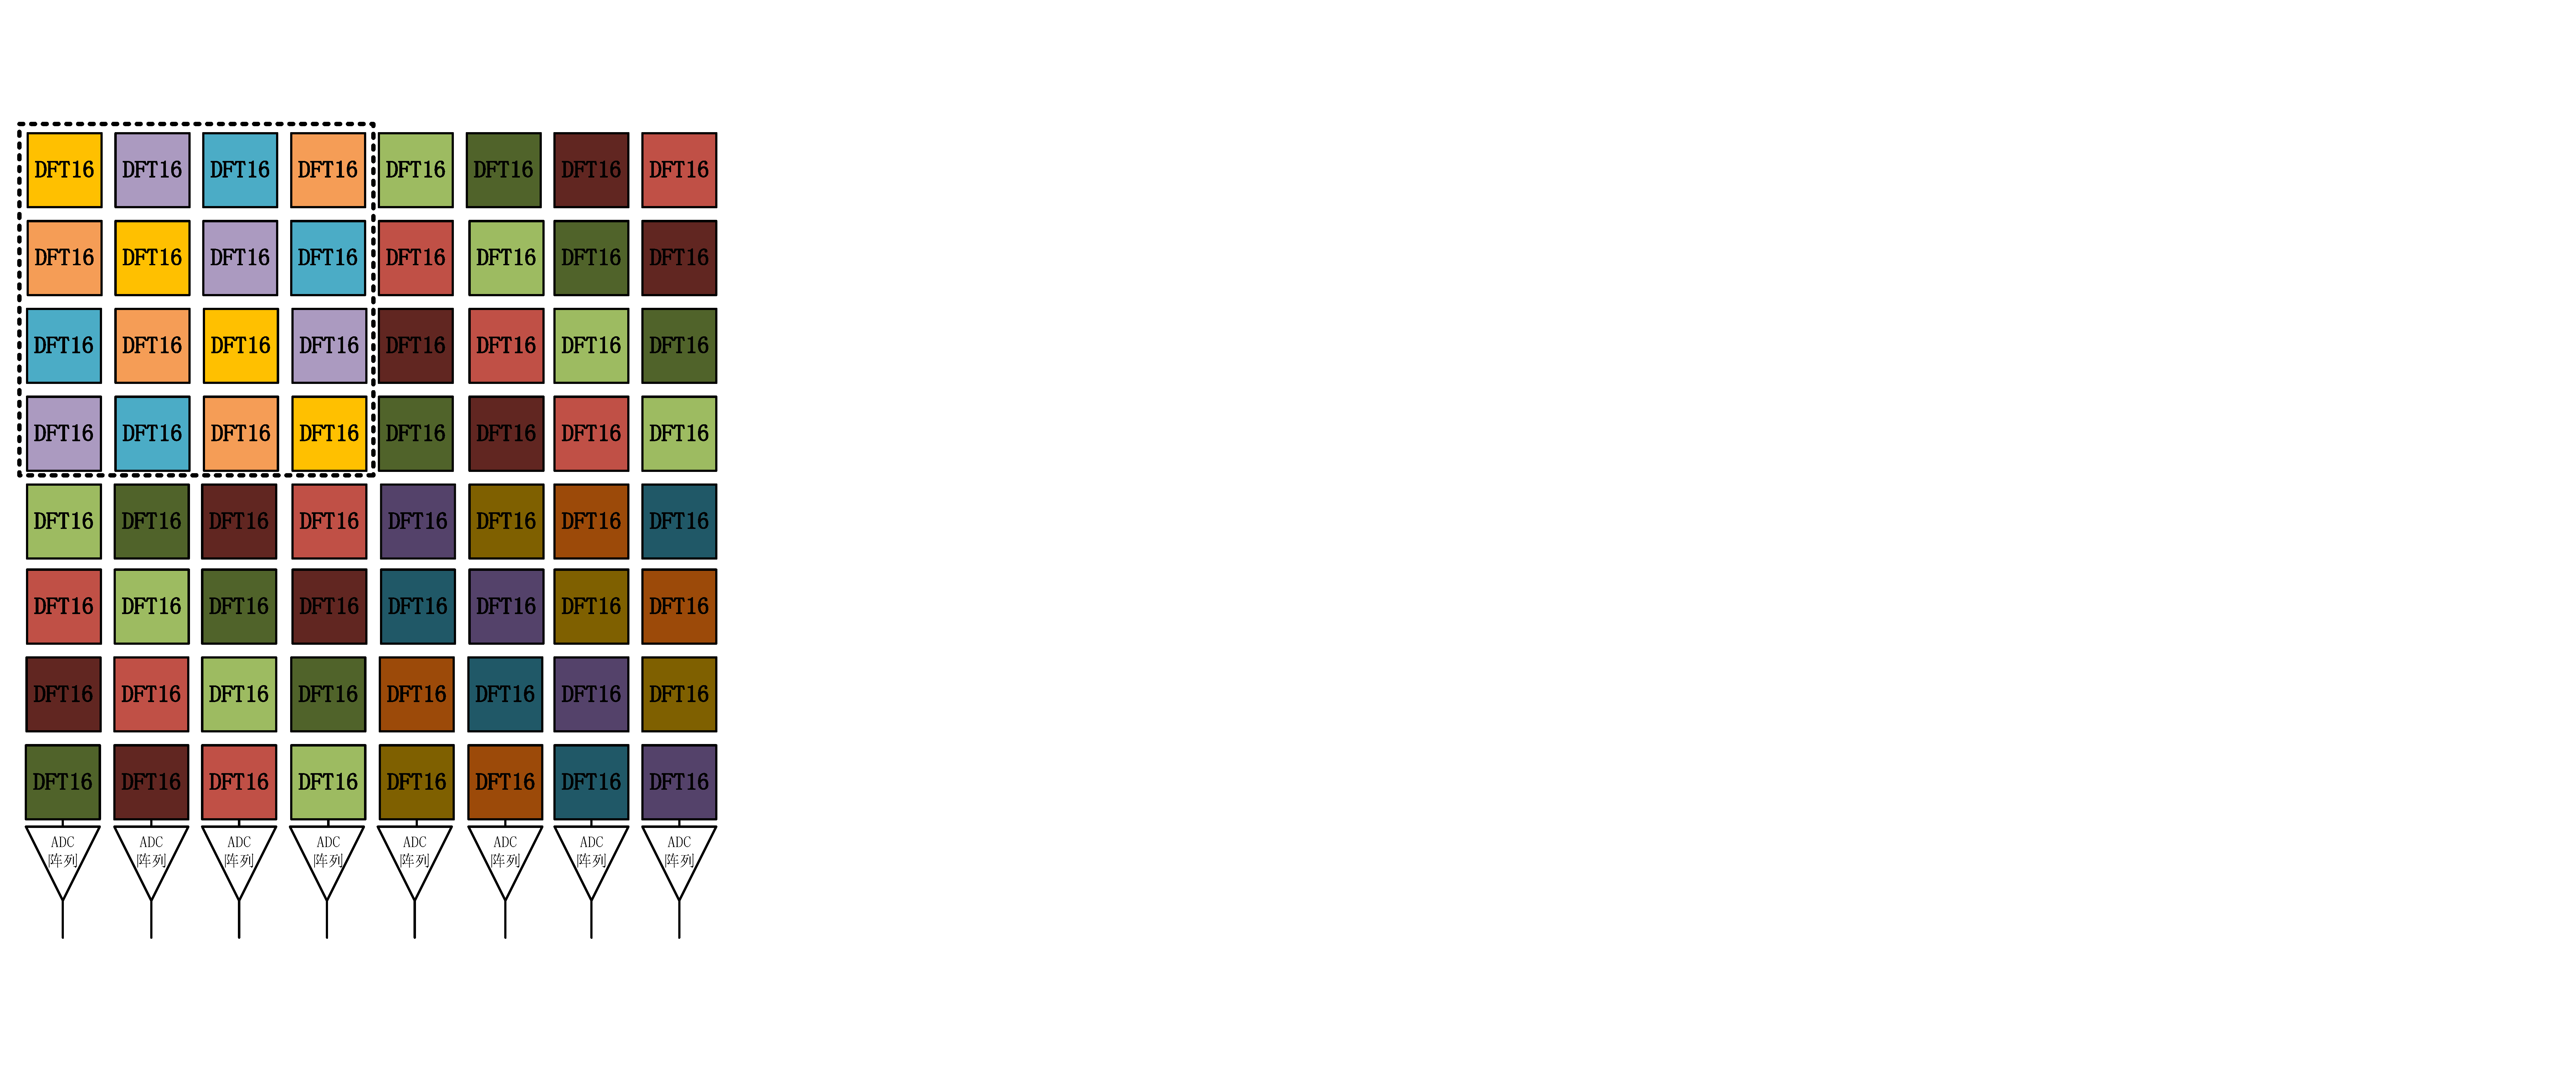
\includegraphics[scale=0.3]{figure/figure3}
\caption{在CIM块中的计算过程}
\end{figure}



\begin{figure}[htbp]
\centering
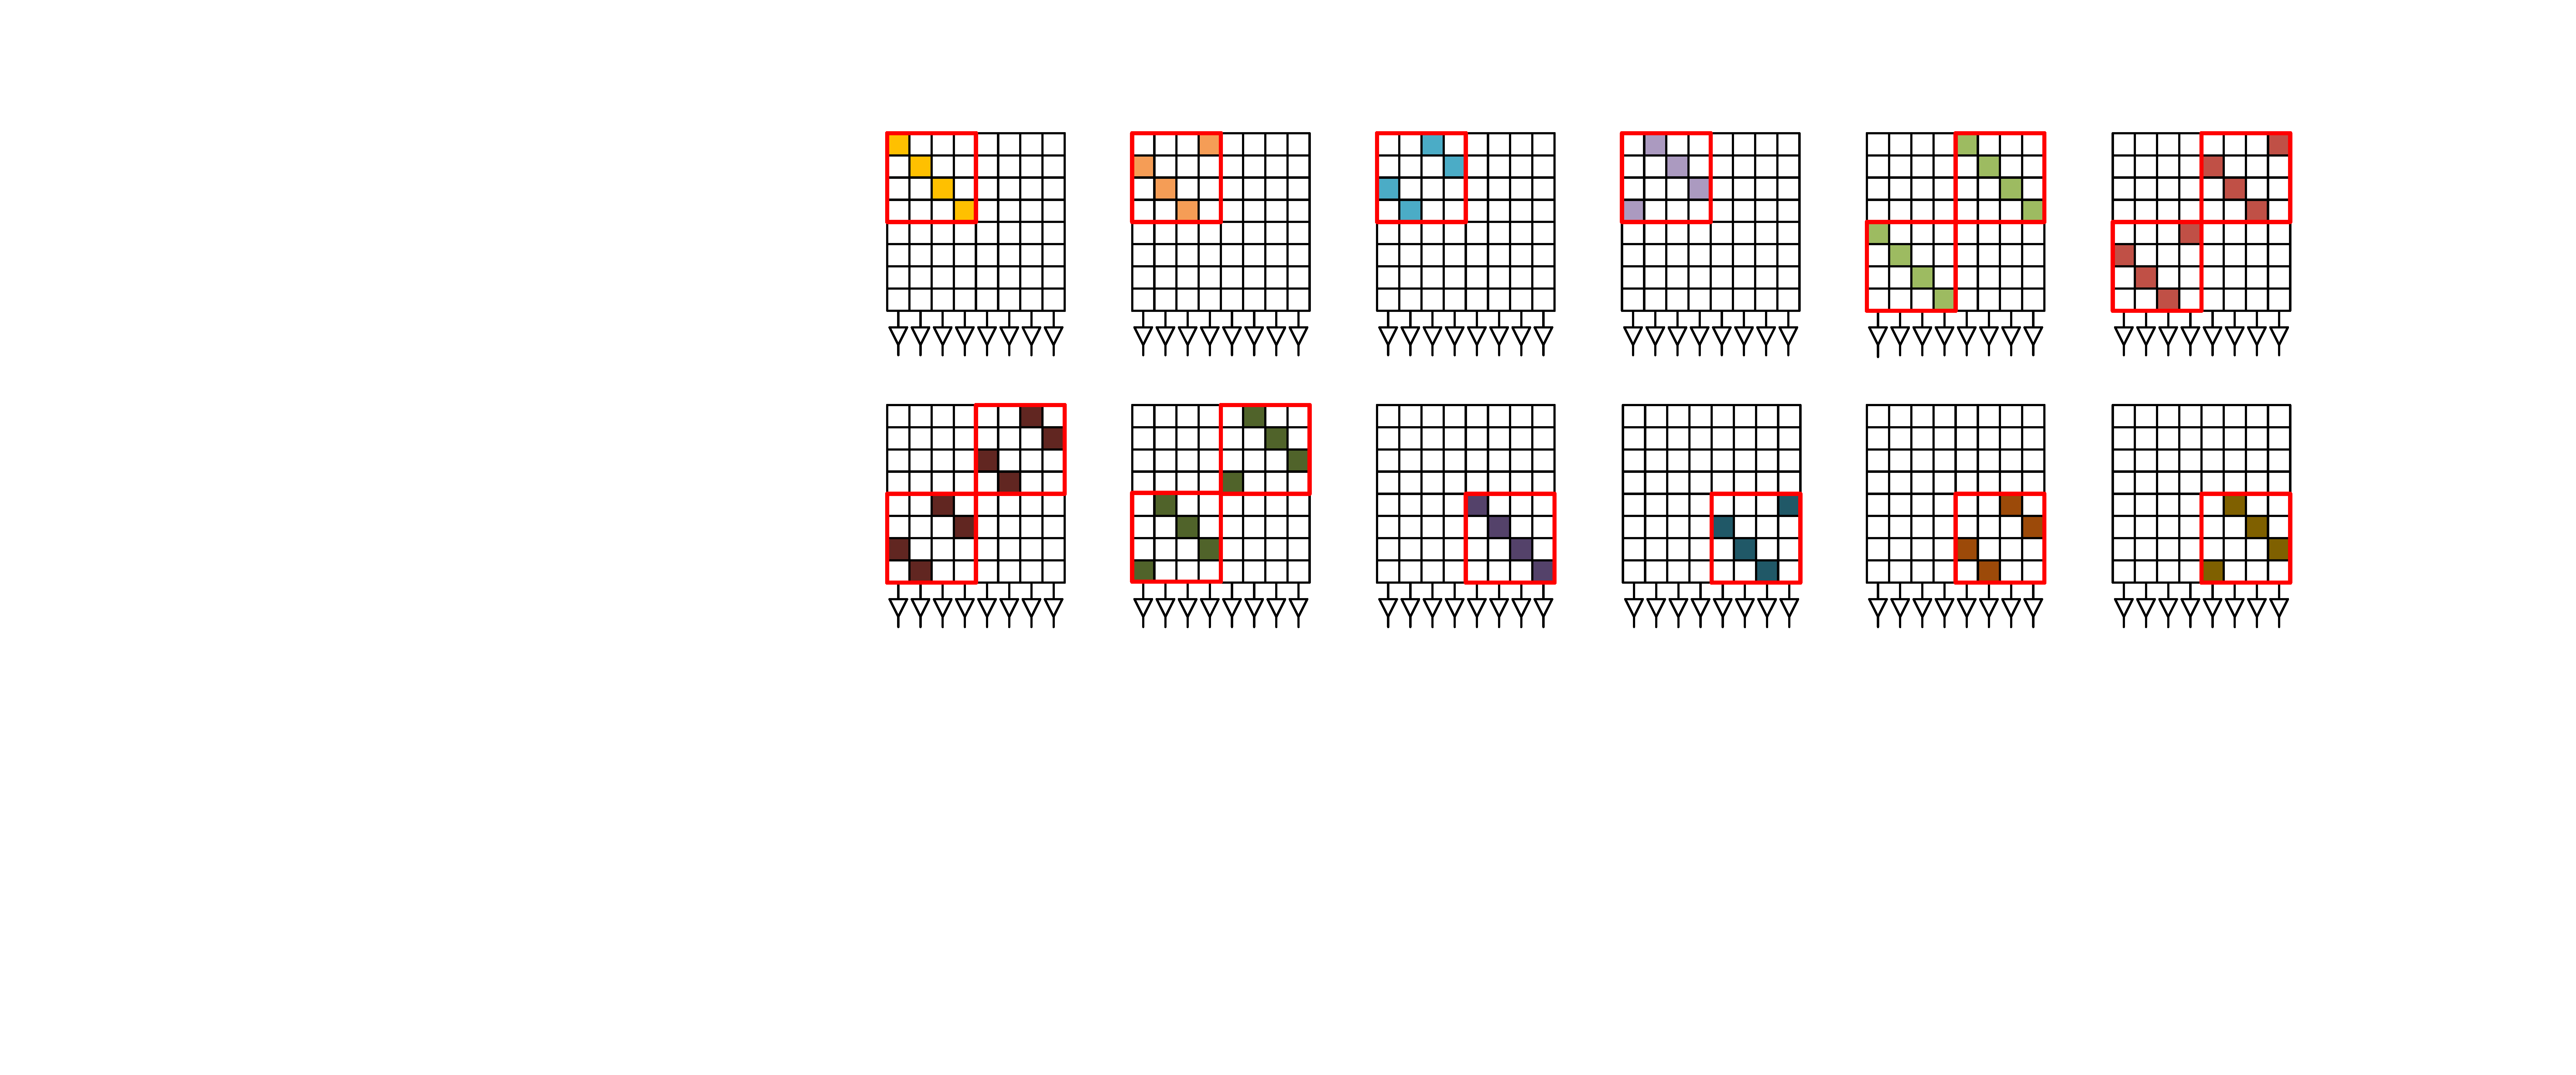
\includegraphics[scale=0.2]{figure/figure4}
\caption{计算时序}
\end{figure}

\end{document} 